
\section{Herleitung der Bewegungsgleichungen}
Als Erstes definieren wir die Positionen der beiden Massepunkte 
\(m_1\) und \(m_2\) des Pendels mithilfe kartesischen Koordinaten 
als (\(x_1\), \(y_1\)) und (\(x_2\), \(y_2\)) gemäss Abbildung \ref{fig:pendulum}.
Wir stellen nun für jede Koordinate die Gleichung über den Winkel auf,
beginnend mit
\begin{align}
    x_1 &= l_1 \sin(\theta_1)\\
    y_1 &= -l_1 \cos(\theta_1).\\
    \shortintertext{Genau dasselbe für}
    x_2 &= l_1 \sin(\theta_1) + l_2 \sin(\theta_2)\\
    y_2 &= -l_1 \cos(\theta_1) - l_2 \cos(\theta_2).  
\end{align}
Hierbei sind \(l_1\) und \(l_2\) die Längen der masselosen Verbindungsstangen.
Danach lässt sich mit der ersten Ableitung der Position von
\(m_1\) nach der Zeit die Geschwindigkeit bestimmen als
\begin{align}
    \dot{x}_1 &= \dot{\theta}_1 l_1 \cos(\theta_1)\\
    \dot{y}_1 &= \dot{\theta}_1 l_1 \sin(\theta_1).\\ 
    \shortintertext{Für den zweiten Massepunkt \(m_2\) gilt}
    \dot{x}_2 &= \dot{\theta}_2 l_2 \cos(\theta_2)
    + \dot{\theta}_1 l_1 \cos(\theta_1)\\
    \dot{y}_2 &= \dot{\theta}_2 l_2 \sin(\theta_2).
\end{align}

\begin{figure}
    \centering
    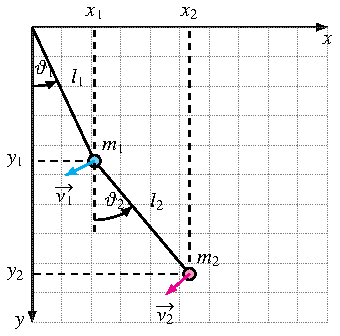
\includegraphics{papers/doppelpendel/images/pendel_pic.pdf}
    \caption{idealisiertes Doppelpendel}
    \label{fig:pendulum}
\end{figure}

\subsection{Aufstellen der Lagrange-Funktion}
Für die Anwendung der Methode von Lagrange müssen wir die Lagrange-Funktion 
\eqref{eq:lagrange} aufstellen.
Dafür stellen wir die Gleichungen der kinetischen und potenziellen Energie auf.
Wir beginnen mit der Energiegleichung für die Masse \(m_1\)
\begin{align}
    T_1 &= \frac{1}{2} m_1 
    \underbrace{( \dot{x}_1^2 + \dot{y}_1^2 )}_{\displaystyle v_1^2}\\
    V_1 &= g m_1 y_1
\end{align}
und ähnlich gilt für die Masse \(m_2\)
\begin{align}
    T_2 &= \frac{1}{2} m_2 
    \underbrace{( \dot{x}_2^2 + \dot{y}_2^2 )}_{\displaystyle v_2^2}\\
    V_2 &= g m_2 y_2
\end{align}
wobei \(g\) die Erdbeschleunigungskonstante ist.
Damit sieht die Gesamtenergie folgendermassen aus:
\begin{align}
    T_{tot} &= T_1 + T_2\\
    V_{tot} &= V_1 + V_2.
\end{align}
Nach einsetzen von \(T_1\) und \(T_2\) ergibt dies
\begin{align}
    T_{tot} &= \frac{1}{2} m_1 ( \dot{x}_1^2 + \dot{y}_1^2 ) +
    \frac{1}{2} m_2 ( \dot{x}_2^2 + \dot{y}_2^2 )\\
    V_{tot} &= g ( m_1 y_1 + m_2 y_2 ).
\end{align}
Das schreiben wir in \(\theta\) um
\begin{align}
    T_{tot} &= \frac{1}{2} m_1 \dot{\theta}^2_1 l_1^2 + 
    \frac{1}{2} m_2 \dot{\theta}^2_2 l_2^2 + \frac{1}{2}
    m_2 \dot{\theta}^2_1 l_1^2 + 
    m_2 \dot{\theta}_1 l_1 \dot{\theta}_2 l_2 
    \cos(\theta_1 - \theta_2)\\
    V_{tot} &= -m_1 g l_1 \cos(\theta_1) -
    m_2 g l_1 \cos(\theta_1) -
    m_2 g l_2 \cos(\theta_2).
\end{align}
Anschliessend setzen wir dies in die Lagrange-Funktion
\begin{align}
    L &= T_{tot} - V_{tot}\\
\end{align}
ein, wobei dies nun
\begin{align}
    L = \frac{1}{2} m_1 \dot{\theta}^2_1 l_1^2 + 
    \frac{1}{2} m_2 \dot{\theta}^2_2 l_2^2 + \frac{1}{2}
    m_2 \dot{\theta}^2_1 l_1^2 + 
    m_2 \dot{\theta}_1 l_1 \dot{\theta}_2 l_2 
    \cos(\theta_1 - \theta_2)\\ \nonumber
    \qquad + m_1 g l_1 \cos(\theta_1) -
    m_2 g l_1 \cos(\theta_1) -
    m_2 g l_2 \cos(\theta_2)
\end{align}
ist.

\subsection{Einsetzen in die Euler-Lagrange Differentialgleichung}
Die im vorherigen Abschnitt definierte Lagrange-Funktion müssen wir in
die Euler-Lagrange Differentialgleichung
\begin{align}
    \label{eq:lag}
    \frac{d}{dt} \left(\frac{\partial L}{\partial \dot{\theta}_1}\right) 
    - \frac{\partial L}{\partial \theta_1} &= 0\\
    \frac{d}{dt} \left(\frac{\partial L}{\partial \dot{\theta}_2}\right) 
    - \frac{\partial L}{\partial \theta_2} &= 0
\end{align}
einsetzen.
Dies lösen wir Schritt für Schritt auf, beginnend mit
\begin{align}
    \frac{\partial L}{\partial \dot{\theta}_1} &= m_1 \dot{\theta}_1 l_1^2
    + m_2 \dot{\theta}_1 l_1^2 + m_2 l_1 l_2 \dot{\theta}_1
    \cos(\theta_1-\theta_2)\\
    \frac{\partial L}{\partial \dot{\theta}_2} &= m_2 \dot{\theta}_2 l_2^2
    + m_2 l_1 l_2 \dot{\theta}_1 \cos(\theta_1-\theta_2).
\end{align}
Danach berechnen wir die Ableitung nach der Zeit
\begin{align}
    \frac{d}{dt} \left(\frac{\partial L}{\partial \dot{\theta}_1}\right) =
    m_1 l_1^2 \ddot{\theta}_1 + m_2 l_1^2 \ddot{\theta}_1\\
    \shortintertext{}
    \qquad + m_2 l_1 l_2 (\ddot{\theta}_2\cos(\theta_1-\theta_2)-
    \dot{\theta}_1 \dot{\theta}_2 \sin(\theta_1-\theta_2) \nonumber\\
    \shortintertext{}
    \qquad + \dot{\theta}_2^2 \sin(\theta_1-\theta_2))
    \nonumber\\
    \shortintertext{}
    \frac{d}{dt} \left(\frac{\partial L}{\partial \dot{\theta}_2}\right) =
    m_2 l_2^2 \ddot{\theta}_2\\
    \shortintertext{}
    \qquad + m_2 l_1 l_2 (\ddot{\theta}_1\cos(\theta_1-\theta_2)+
    \dot{\theta}_1 \dot{\theta}_2 \sin(\theta_1-\theta_2) \nonumber\\
    \shortintertext{}
    \qquad - \dot{\theta}_1^2 \sin(\theta_1-\theta_2))
    \nonumber
\end{align}
und zuletzt
\begin{align}
    \frac{\partial L}{\partial {\theta}_1} &= -m_1 l_1 l_2 \dot{\theta}_1
    \dot{\theta}_2 \sin(\theta_1-\theta_2) - m_1 g l_1 \sin(\theta_1)
    - m_2 g l_1 \sin(\theta_1)\\
    \frac{\partial L}{\partial {\theta}_2} &= m_2 l_1 l_2 \dot{\theta}_1
    \dot{\theta}_2 \sin(\theta_1-\theta_2) - m_2 g l_2 \sin(\theta_2).
\end{align}
Wir verfolgen das Ziel nach \(\ddot{\theta}_1\) und \(\ddot{\theta}_2\) aufzulösen.
Dafür formen wir die Gleichung \eqref{eq:lag} folgendermassen um:
\begin{align}
    \frac{d}{dt} \left(\frac{\partial L}{\partial \dot{\theta}_1}\right) 
    = \frac{\partial L}{\partial \theta_1}\\
    \frac{d}{dt} \left(\frac{\partial L}{\partial \dot{\theta}_2}\right) 
    = \frac{\partial L}{\partial \theta_2}.
\end{align}
Hier setzen wir nun die vorher ausgerechneten Terme ein und erhalten nach wenigen
Umformungen die Differentialgleichung für \(\theta_1\)
\begin{align}
    \ddot{\theta}_1 l_1^2 (m_1 + m_2) \, = -m_1 g l_1 \sin(\theta_1) - m_2 g l_1 \sin(\theta_1)\\
    \qquad - m_2 l_1 l_2 \left(\ddot{\theta}_2 \cos(\theta_1-\theta_2) 
    + \dot{\theta}_2^2 \sin(\theta_1-\theta_2) \right) \nonumber
    \shortintertext{und die Differentialgleichung für \(\theta_2\)}
    m_2 l_2^2 \ddot{\theta_2} = -m_2 g l_2 \sin(\theta_2)\\
    \qquad - m_2 l_1 l_2 \left(\ddot{\theta}_1 \cos(\theta_1-\theta_2) 
    - \dot{\theta}_1^2 \sin(\theta_1-\theta_2) \right). \nonumber
\end{align}
Nun können wir die Gleichung endlich nach \(\ddot{\theta}_1\) und \(\ddot{\theta}_2\) auflösen und erhalten
\begin{align}
    \label{eq:bewegungsgleichung1}
    \ddot{\theta}_1 &= -\frac{g}{l_1} \sin(\theta_1) - \frac{m_2}{m_1+m_2} \frac{l_2}{l_1} 
    \left(\ddot{\theta}_2 \cos(\theta_1-\theta_2) + \dot{\theta}_2^2 \sin(\theta_1-\theta_2) \right)\\
    \ddot{\theta}_2 &= -\frac{g}{l_2} \sin(\theta_2) - \frac{l_1}{l_2} 
    \left(\ddot{\theta}_1 \cos(\theta_1-\theta_2) - \dot{\theta}_1^2 \sin(\theta_1-\theta_2) \right)
\end{align}
als Lösung.

An dieser Stelle können wir unser Ergebnis plausibilisieren, indem wir in
\(\ddot{\theta}_1\) die Länge \(l_2=0\) setzen
\begin{align}
    \lim_{l_2 \to 0} \ddot{\theta}_1 &= -\frac{g}{l_1} \sin(\theta_1).
\end{align}
Physikalisch bedeutet das eine Verkleinerung des zweiten Stabs bis dieser verschwindet und
das Doppelpendel zu einem einfachen transformiert.
Man sieht wie dabei der rechte Term der Gleichung \eqref{eq:bewegungsgleichung1} vollständig
wegfällt und übrig bleibt, wie vermutet, die Bewegungsgleichung des einfachen Pendels.
Parallel gilt das auch für \(\ddot{\theta}_2\) wenn die Länge \(l_1=0\) gesetzt wird
\begin{align}
    \lim_{l_1 \to 0} \ddot{\theta}_2 &= -\frac{g}{l_2} \sin(\theta_2).
\end{align}

\subsection{Anfangsbedingungen}
Als Ergebnis erhalten wir für \(\theta\) jeweils eine Differentialgleichung zweiter Ordnung.
Diese lassen sich nicht analytisch nach der Zielvariable auflösen,
d.h. man erhält keine Funktion für die Position in Abhängigkeit von \(\theta\) 
wie beispielsweise für das einfache Pendel. 

Trotzdem lassen sich mit Anfangsbedingungen für beide Winkel numerische Lösungen ermitteln.
Dazu muss man für \(\theta_1(t=0)\) und \(\theta_2(t=0)\), welches die Anfangspositionen darstellen,
einen Wert definieren wie z.B. jeweils 20°. Genauso für die Anfangsgeschwindigkeiten \(\dot{\theta}_1(t=0)\)
und \(\dot{\theta}_2(t=0)\).
Diese werden meistens mit 0 festgelegt. Man kann sich das vorstellen, als würde man das Pendel
am zweiten Massepunkt fassen auf die Position ziehen wo beide Winkel 20° betragen und dann loslassen.
Anhand der numerischen Lösungen lassen sich bereits Simulationen erstellen, da der Computer
sowiese auf diskrete Werte angewiesen ist macht das keinen Unterschied.
Mit den Simulationen könnte man beispielsweise das chaotische Verhalten des Pendels bei verschiedenen 
Anfangsbedingungen genauer analysieren.

